\documentclass{article}

\usepackage{postprocess/context/arxiv}

\usepackage[utf8]{inputenc} % allow utf-8 input
\usepackage{amsmath}
\usepackage[T1]{fontenc}    % use 8-bit T1 fonts
\usepackage{hyperref}       % hyperlinks
\usepackage{url}            % simple URL typesetting
\usepackage{booktabs}       % professional-quality tables
\usepackage{amsfonts}       % blackboard math symbols
\usepackage{nicefrac}       % compact symbols for 1/2, etc.
\usepackage{microtype}      % microtypography
\usepackage{graphicx}
\usepackage{natbib}
\usepackage{doi}
\usepackage{float}
\usepackage{subcaption}
\usepackage{wrapfig}

\title{Causal Discovery Report on Abalone}

\author{ \href{https://orcid.org/0000-0000-0000-0000}{
\includegraphics[scale=0.06]{postprocess/context/orcid.pdf}\hspace{1mm}Causal Copilot}}

\renewcommand{\headeright}{Technical Report}
\renewcommand{\undertitle}{Technical Report}

\hypersetup{
pdftitle={Causal Discovery Report on Abalone},
pdfauthor={Causal Copilot},
pdfkeywords={Causal Discovery, Large Language Model, PC, Abalone},
}

\begin{document}
\maketitle

\begin{abstract}
This report analyzes the Abalone dataset, which includes physical characteristics and age variables of abalones. Using a combination of data preprocessing and causal discovery algorithms assisted by a large language model, we selected the PC, GES, and NOTEARS algorithms based on their suitability for handling the dataset's statistical properties. Our findings reveal complex causal relationships, with age influencing physical dimensions such as diameter and weight, while length impacts both shell and shucked weight. Key contributions of this work include validating the interdependencies between growth variables and providing insights for ecological and commercial applications, despite acknowledging varying levels of reliability in the causal links identified. The incorporation of expert knowledge and statistical analysis enhances our understanding of abalone biology and informs future research directions.
\end{abstract}

\keywords{Causal Discovery, Large Language Model, PC, Abalone}

\raggedbottom
\section{Introduction}
The Abalone dataset features a collection of variables that capture the physical characteristics and age of abalones, a type of marine mollusk. Key variables such as age, length, diameter, height, and various weights provide insights into the growth patterns and health of these organisms. Specifically, age is a significant determinant of size dimensions, which in turn influence overall weight measures. Understanding the causal relationships among these variables is crucial for several applications, including ecological studies and commercial practices. Additionally, growth patterns can be impacted by environmental factors and biological relationships, further complicating the analysis. This report aims to explore these causal connections using the available data, contributing valuable insights to the understanding of abalone biology and the implications for their management and sustainability.

\section{Background Knowledge}
\subsection{Detailed Explanation about the Variables}
\begin{itemize}
\item \textbf{Age}: This variable indicates the age of the abalone, typically measured in years. It can be derived from growth rings observed on the shell or other biological markers. Age significantly influences various physical characteristics of the abalone, as these features are expected to change with maturation and growth.

\item \textbf{Length}: This variable measures the longest dimension of the abalone's shell, usually recorded in millimeters. Length serves as a primary indicator of growth and maturity, as larger abalones generally exhibit greater lengths.

\item \textbf{Diameter}: This variable refers to the width of the shell, also measured in millimeters. Like length, diameter is a key dimension that reflects the size of the abalone's shell, and it may correlate closely with age.

\item \textbf{Height}: This variable measures the vertical dimension of the shell and contributes an additional perspective on the overall size of the abalone. Height, along with length and diameter, can serve as an important marker of the abalone's health and growth status.

\item \textbf{Shell weight}: This variable refers to the weight of the shell alone, typically measured in grams. Shell weight can reflect the density, strength, and condition of the shell, all of which may evolve as the abalone ages and grows.

\item \textbf{Whole weight}: This variable represents the total weight of the abalone, encompassing all components, including shell and meat. Whole weight serves as a crucial measure of the abalone's overall size and health.

\item \textbf{Shucked weight}: This variable denotes the weight of the abalone's meat once it has been extracted from the shell. Shucked weight is significant for commercial purposes, as it indicates the quantity of product available for consumption.

\item \textbf{Viscera weight}: This variable represents the weight of the internal organs of the abalone, contributing to the comprehensive weight measurement. Viscera weight can offer insights into the health and maturity level of the abalone.
\end{itemize}

\subsection{Possible Causal Relations among these Variables}

\begin{minipage}[t]{0.7\linewidth}
\begin{itemize}
    \item \textbf{Age $\rightarrow$ Length}: As abalones age, they typically grow in size, leading to an increase in the length of their shells.
    
    \item \textbf{Age $\rightarrow$ Diameter}: The aging process results in an increase in the diameter of the abalone's shell as it matures and grows.
    
    \item \textbf{Age $\rightarrow$ Height}: Similarly, age is expected to influence the height of the shell, with older abalones generally exhibiting greater height due to growth.
    
    \item \textbf{Length $\rightarrow$ Whole weight}: An increase in shell length likely results in a corresponding increase in the whole weight of the abalone, as larger shells contain more biomass.
    
    \item \textbf{Diameter $\rightarrow$ Whole weight}: As the diameter of the shell increases, the whole weight of the abalone also tends to increase due to the larger volume.
    
    \item \textbf{Height $\rightarrow$ Whole weight}: An increase in shell height is likely associated with greater whole weight, reflecting the overall growth of the abalone.
    
    \item \textbf{Length $\rightarrow$ Shell weight}: Greater length typically leads to an increase in shell weight, as larger shells are heavier due to their size and structure.
    
    \item \textbf{Diameter $\rightarrow$ Shell weight}: An increase in the diameter of the shell contributes positively to the shell weight, as a wider shell is more substantial.
    
    \item \textbf{Height $\rightarrow$ Shell weight}: An increase in height is expected to correlate with an increase in shell weight, indicative of the shell's overall mass.
    
    \item \textbf{Whole weight $\rightarrow$ Shucked weight}: The total weight of the abalone influences the weight of the meat after being shucked, as larger whole abalones generally yield more meat.
    
    \item \textbf{Age $\rightarrow$ Shucked weight}: As abalones mature and grow older, their shucked weight is likely to increase, reflecting the increase in meat available for consumption.
    
    \item \textbf{Age $\rightarrow$ Viscera weight}: Over time, as abalones age, their viscera weight typically increases, indicating growth and development of internal organs.
    
    \item \textbf{Whole weight $\rightarrow$ Viscera weight}: A higher whole weight correlates with increased viscera weight, as a larger abalone generally has more substantial internal organs.
    
    \item \textbf{Shell weight $\rightarrow$ Viscera weight}: The weight of the shell may also influence the viscera weight, as heavier shells might correlate with healthier and larger internal organs.
\end{itemize}
\end{minipage}
\hspace{0.05\textwidth}
\begin{minipage}[t]{0.3\linewidth}
\begin{figure}[H]
    \centering
    \resizebox{\linewidth}{!}{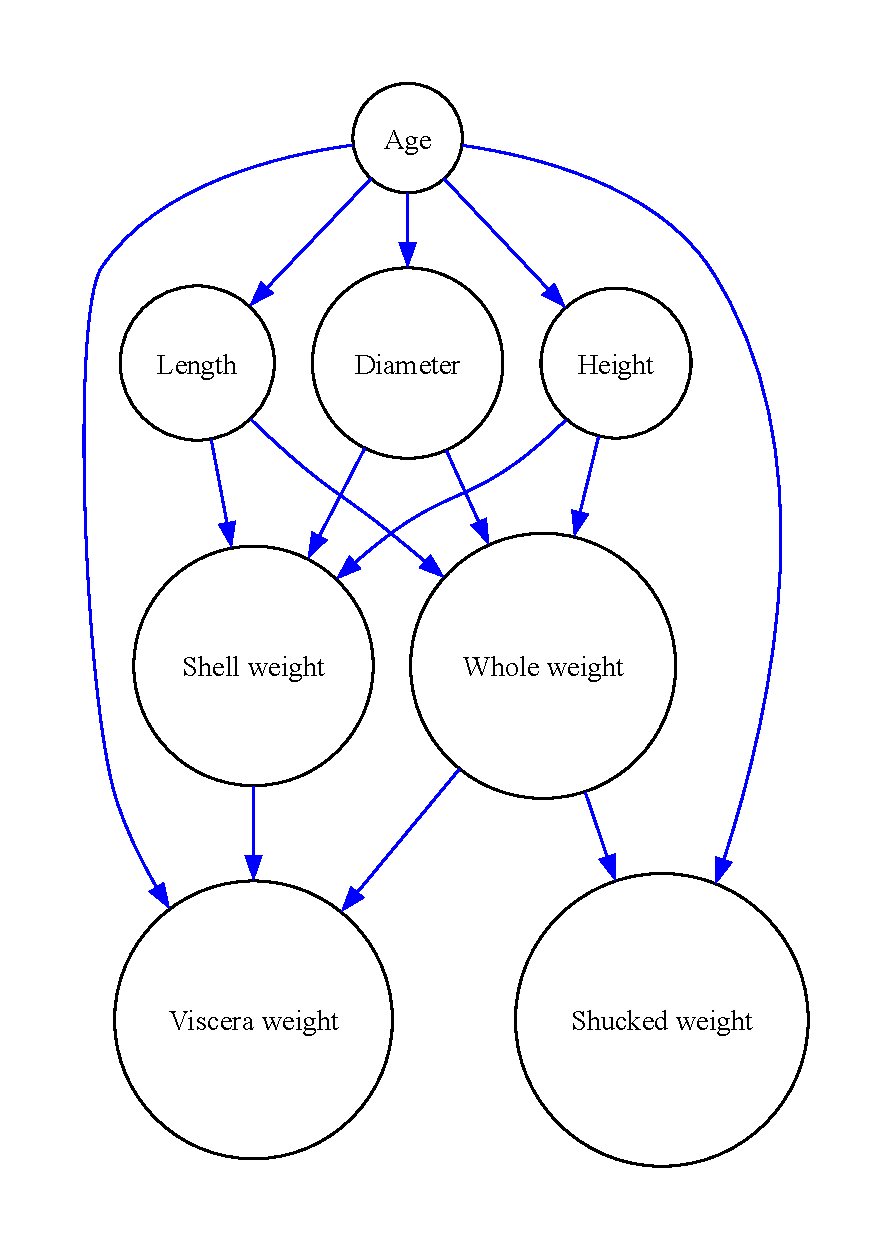
\includegraphics[height=0.3\textheight]{./demo_data/20241104_132155/Abalone/output_graph/potential_relation.pdf}}
    \caption{\label{fig:relation}Possible Causal Relation Graph}
\end{figure}
\end{minipage}

\section{Dataset Descriptions and EDA}
The following is a preview of our original dataset.

\begin{table}[H]
    \centering
    \caption{Dataset Preview}
    \begin{tabular}{rrrrrrrr}
\toprule
 Age &  Length &  Shell weight &  Diameter &  Height &  Whole weight &  Shucked weight &  Viscera weight \\
\midrule
15.0 &   0.455 &         0.365 &     0.095 &  0.5140 &        0.2245 &          0.1010 &           0.150 \\
 7.0 &   0.350 &         0.265 &     0.090 &  0.2255 &        0.0995 &          0.0485 &           0.070 \\
 9.0 &   0.530 &         0.420 &     0.135 &  0.6770 &        0.2565 &          0.1415 &           0.210 \\
10.0 &   0.440 &         0.365 &     0.125 &  0.5160 &        0.2155 &          0.1140 &           0.155 \\
 7.0 &   0.330 &         0.255 &     0.080 &  0.2050 &        0.0895 &          0.0395 &           0.055 \\
\bottomrule
\end{tabular}

\end{table}

\subsection{Data Properties}
We employ several statistical methods to identify data properties.

The shape of the data, data types, and missing values are assessed directly from the dataframe.
Linearity is evaluated using Ramsey’s RESET test, followed by the Benjamini \& Yekutieli procedure for multiple test correction.
Gaussian noise is assessed through the Shapiro-Wilk test, also applying the Benjamini \& Yekutieli procedure for multiple test correction.
Time-Series and Heterogeneity are derived from user queries.

Properties of the dataset we analyzed are listed below.

\begin{table}[H]
    \centering
    \caption{Data Properties}

        \begin{tabular}{rrrrrrrr}
            \toprule
            Shape ($n$ x $d$) & Data Type & Missing Value & Linearity & Gaussian Errors & Time-Series & Heterogeneity \\
            \midrule
            (4177, 8)   & Continuous & False & True & True & False & False \\
            \bottomrule
        \end{tabular}
        
\end{table}


\subsection{Distribution Analysis}
The following figure shows distributions of different variables. The orange dash line represents the mean, 
and the black line represents the median. Variables are categorized into three types according to their distribution characteristics.

\begin{figure}[H]
\centering
\includegraphics[width=\linewidth]{./demo_data/20241104_132155/Abalone/output_graph/eda_dist.jpg}
\caption{\label{fig:dist}Distribution Plots of Variables}
\end{figure}

\begin{itemize}
\item Slight left skew distributed variables: Length, Shell Weight, Diameter, Whole Weight
\item Slight right skew distributed variables: Age, Height, Shucked Weight, Viscera Weight
\item Symmetric distributed variables: None
\end{itemize}

\subsection{Correlation Analysis}

\begin{minipage}[t]{0.5\linewidth}
    In this analysis, we will categorize the correlation statistics of features in the dataset into three distinct categories: Strong correlations, Moderate correlations, and Weak correlations.

\begin{itemize}
\item Strong Correlated Variables: Shell weight and Length, Height and Whole weight, Height and Shucked weight, Viscera weight and Shell weight, Viscera weight and Height, Viscera weight and Shucked weight
\item Moderate Correlated Variables: Length and Age, Shell weight and Age, Diameter and Age, Height and Age, Diameter and Length, Diameter and Shell weight, Whole weight and Diameter, Shucked weight and Age, Shucked weight and Length, Shucked weight and Diameter, Whole weight and Height, Whole weight and Shell weight
\item Weak Correlated Variables: None
\end{itemize}
\vfill
\end{minipage}
\hfill
\begin{minipage}[t]{0.5\linewidth}
    \begin{figure}[H]
        \centering
        \vspace{-1.5cm}
        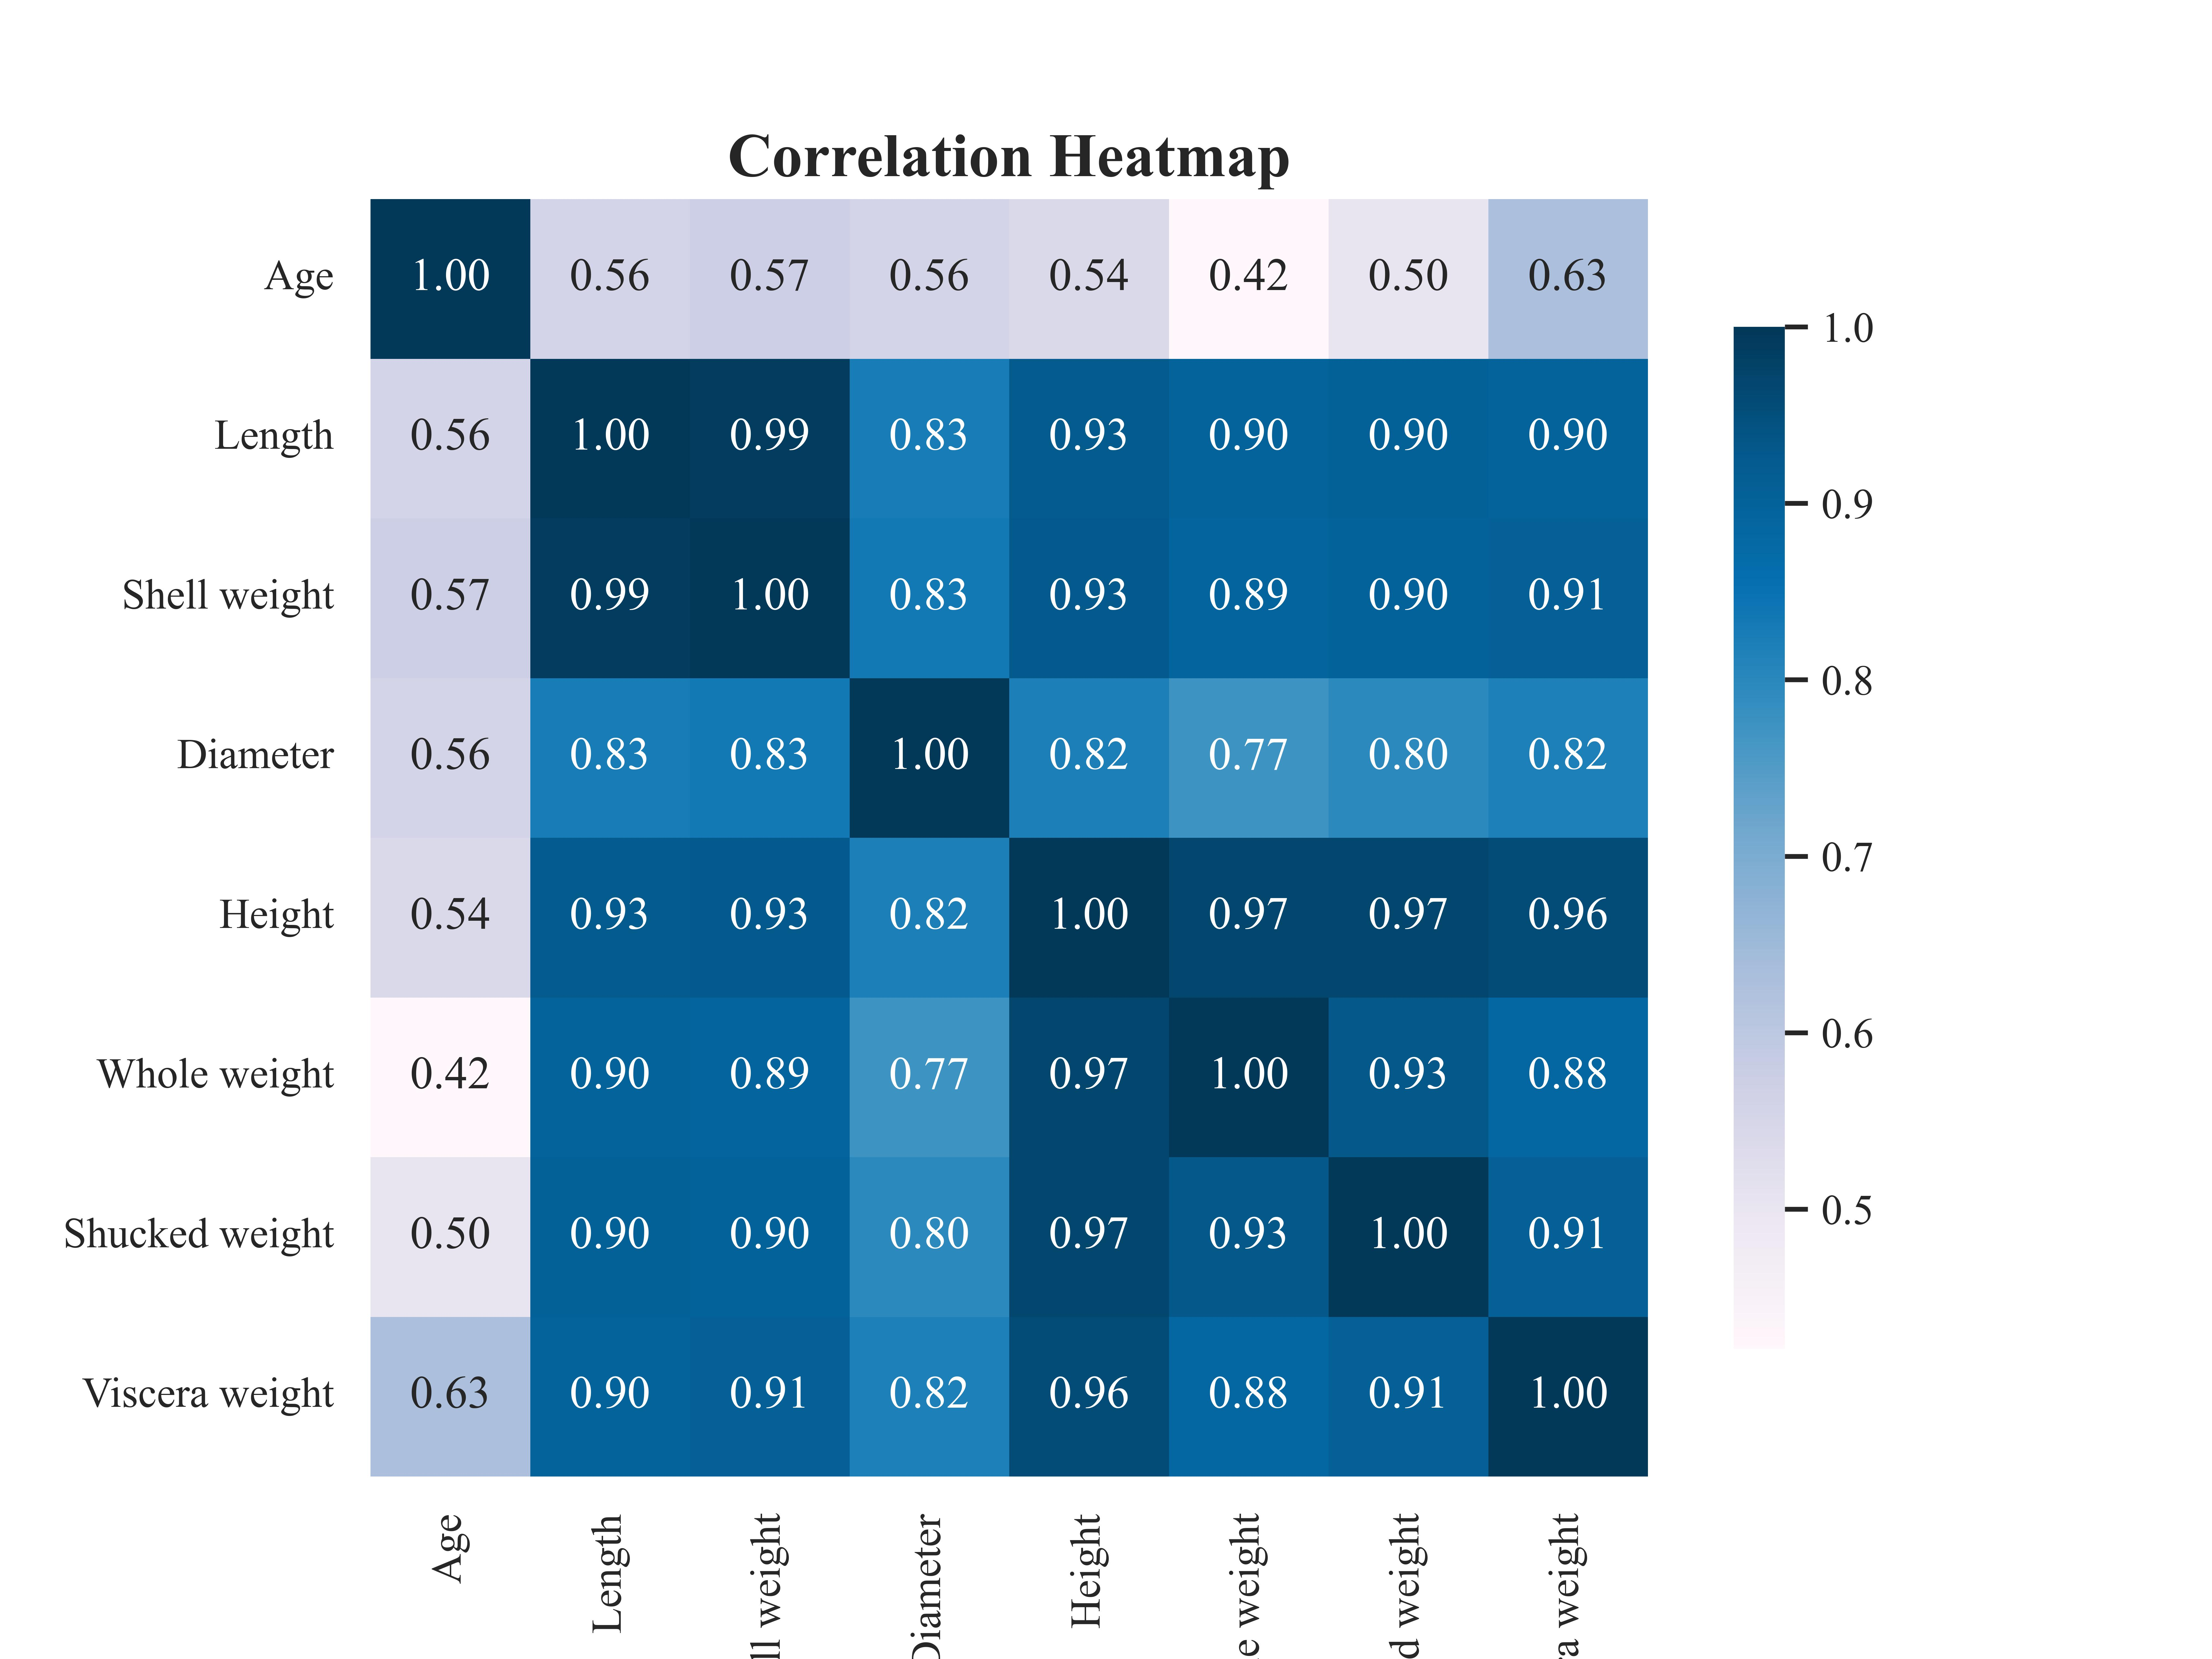
\includegraphics[width=\linewidth]{./demo_data/20241104_132155/Abalone/output_graph/eda_corr.jpg}
        \caption{\label{fig:corr}Correlation Heatmap of Variables}
    \end{figure}
\end{minipage}

\section{Discovery Procedure}

In this section, we provide a detailed description of the causal discovery process implemented by Causal Copilot. 
We also provide the chosen algorithms and hyperparameters, along with the justifications for these selections.

\subsection{Data Preprocessing}
In this initial step, we preprocessed the data and examined its statistical characteristics. 
This involved cleaning the data, handling missing values, and performing exploratory data analysis to understand distributions and relationships between variables.
                
\subsection{Algorithm Selection assisted with LLM}
Following data preprocessing, we employed a large language model (LLM) to assist in 
selecting appropriate algorithms for causal discovery based on the statistical characteristics of the dataset and relevant background knowledge. 
The top three chosen algorithms, listed in order of suitability, are as follows:   
        
\begin{itemize}

\item \textbf{PC}:
\begin{itemize}
    \item \textbf{Description}: The PC algorithm is a constraint-based method that learns the structure of a causal graph from data by testing conditional independencies between variables, producing a directed acyclic graph (DAG).
    \item \textbf{Justification}: The dataset is large (4177 samples) with all relevant variables observed, making PC advantageous due to its efficiency in handling large datasets and its ability to quickly prune unnecessary edges.
\end{itemize}

\item \textbf{GES}:
\begin{itemize}
    \item \textbf{Description}: Greedy Equivalence Search (GES) is a score-based causal discovery algorithm that identifies the optimal causal structure by navigating the space of equivalence classes of Directed Acyclic Graphs (DAGs) using a score function.
    \item \textbf{Justification}: The dataset follows predominantly linear relationships, allowing GES to provide a robust and efficient method for causal discovery, especially since it operates under the assumption of no hidden confounders.
\end{itemize}

\item \textbf{NOTEARS}:
\begin{itemize}
    \item \textbf{Description}: NOTEARS transforms the problem of learning Directed Acyclic Graphs (DAGs) into a continuous optimization problem, suitable for high-dimensional data.
    \item \textbf{Justification}: Given the continuous nature of the variables and the sizable dataset, NOTEARS is a practical option, especially if the researcher is looking for a method that can efficiently handle large-scale and potentially nonlinear structures.
\end{itemize}

\end{itemize}
                    

\subsection{Hyperparameter Values Proposal assisted with LLM}
Once the algorithms were selected, the LLM aided in proposing hyperparameters 
for the chosen algorithm, which are specified below:
        
\begin{itemize}

\item \textbf{alpha}:
\begin{itemize}
    \item \textbf{Value}: 0.05
    \item \textbf{Explanation}: Given the sample size of 4177, which falls in the range of 500-10000, the suggested value of 0.05 is appropriate. This strikes a balance between Type I error control and retaining statistical power, making it suitable for analyzing continuous data with predominantly linear relationships.
\end{itemize}

\item \textbf{findep\_test}:
\begin{itemize}
    \item \textbf{Value}: fisherz
    \item \textbf{Explanation}: Since the dataset consists of continuous variables and the relationships are predominantly linear with Gaussian errors, using Fisher's Z test is appropriate. It aligns with the assumptions of linearity and Gaussianity present in the data.
\end{itemize}

\item \textbf{depth}:
\begin{itemize}
    \item \textbf{Value}: -1
    \item \textbf{Explanation}: The dataset has 8 features, which is relatively small. Using an unrestricted depth of -1 allows for a comprehensive exploration of the dependencies among variables without imposing unnecessary limitations, thus maximizing the accuracy of the causal discovery.
\end{itemize}

\end{itemize}

\subsection{Graph Tuning with Bootstrap and LLM Suggestion}
In the final step, we performed graph tuning with suggestions provided by the Bootstrap and LLM.
            
Firstly, we use the Bootstrap technique to get how much confidence we have on each edge in the initial graph.
If the confidence probability of a certain edge is greater than 95\% and it is not in the initial graph, we force it.
Otherwise, if the confidence probability is smaller than 5\% and it exists in the initial graph, we change it to the edge type with the highest probability.
            
After that, We utilize LLM to help us prune edges and determine the direction of undirected edges according to its knowledge repository.
In this step LLM can use background knowledge to add some edges that are neglected by Statistical Methods.
Voting techniques are used to enhance the robustness of results given by LLM, and the results given by LLM should not change results given by Bootstrap.

By integrating insights from both of Bootstrap and LLM to refine the causal graph, we can achieve improvements in graph's accuracy and robustness.
            

\section{Results Summary}

\subsection{Initial Graph}

\begin{figure}[H]
    \centering
    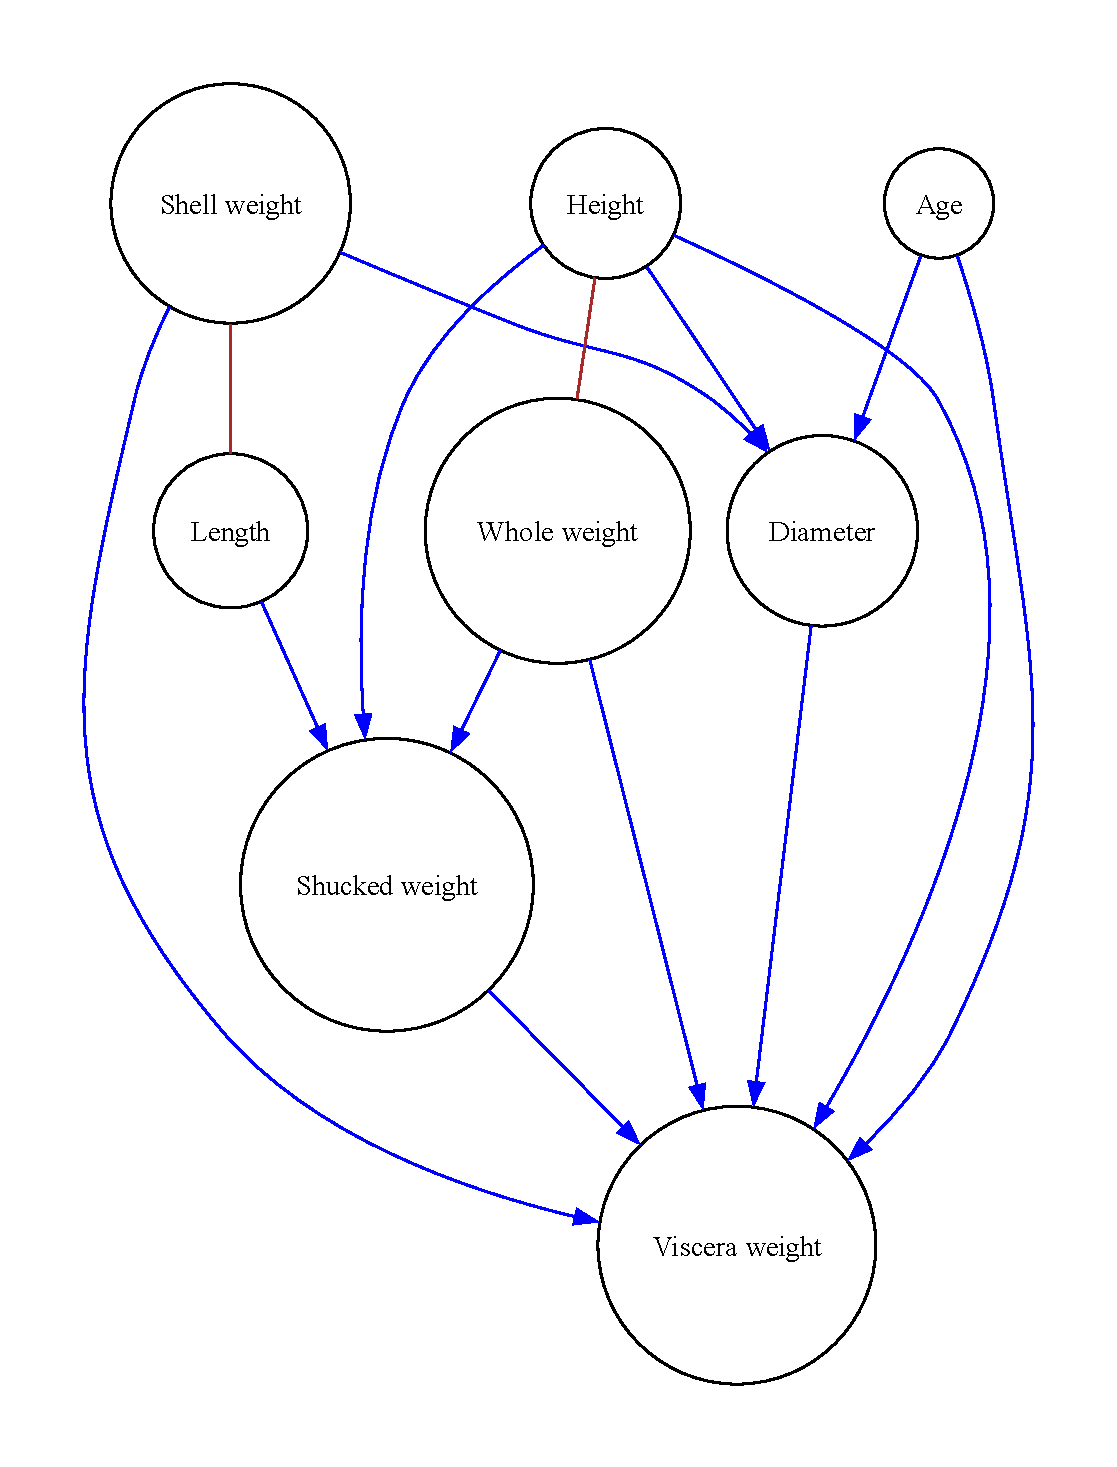
\includegraphics[height=0.3\textheight]{./demo_data/20241104_132155/Abalone/output_graph/initial_graph.pdf}
    \caption{Initial Graph}
\end{figure}

The above is the initial result graph produced by our algorithm.

The causal relationships among the variables indicate a complex interplay in growth and physical characteristics. Age influences both Diameter and Viscera weight, suggesting that as an organism ages, it develops larger body dimensions and increased organ mass. Length has a reciprocal causative effect on Shell weight, while also impacting Shucked weight, indicating that the overall size plays a crucial role in determining shell formation and the weight of the edible tissue. Moreover, Shell weight contributes to Diameter and Viscera weight, reflecting how the physical structure of the organism is associated with its internal growth. Height also significantly impacts Diameter and various weight measures, such as Whole weight and Shucked weight, demonstrating that taller organisms tend to have larger diameters and greater overall mass. Lastly, Whole weight reciprocally affects Height and also influences Shucked and Viscera weight, indicating that overall biomass affects both physical stature and the organic content within. The interconnectedness of these variables suggests a robust model of growth where age, size, and weight metrics are mutually influential.

\subsection{Revised Graph}

\begin{minipage}[t]{0.6\linewidth}
    
        By using the method mentioned in the Section 4.4, we provide a revised graph pruned with Bootstrap and LLM suggestion.
        Pruning results are as follows.
        
        Bootstrap doesn't force or forbid any edges.
            
        The following are force results given by LLM:
            
        \begin{itemize}
            
            \item \textbf{Age $\rightarrow$ Length}: As abalones age, they typically grow in size, leading to an increase in length.
                
            \item \textbf{Age $\rightarrow$ Shell weight}: Older abalones have heavier shells as they develop and grow, resulting in an increase in shell weight over time.
                
            \item \textbf{Age $\rightarrow$ Height}: With age, abalones generally increase in size, including height, as they mature and grow.
                
            \item \textbf{Age $\rightarrow$ Whole weight}: As abalones age, their overall mass increases, contributing to a greater whole weight.
                
            \item \textbf{Age $\rightarrow$ Shucked weight}: An increase in age usually corresponds with more developed and larger meat, thereby increasing shucked weight.
                
            \item \textbf{Length $\rightarrow$ Diameter}: As the length of the abalone increases, the diameter also tends to increase, reflecting their overall growth in size.
                
            \item \textbf{Length $\rightarrow$ Height}: Similarly, increases in length are associated with increases in height as the abalone's dimensions expand with growth.
                
            \item \textbf{Length $\rightarrow$ Whole weight}: A larger length typically indicates a larger whole weight, as the mass of the abalone increases with size.
                
            \item \textbf{Length $\rightarrow$ Viscera weight}: As length increases, the viscera weight may also increase due to more developed internal organs corresponding with larger body size.
                
            \item \textbf{Shell weight $\rightarrow$ Whole weight}: The weight of the shell contributes directly to the total weight of the abalone, establishing a clear causal relationship.
                
            \item \textbf{Shell weight $\rightarrow$ Shucked weight}: Heavier shells usually correspond to greater quantities of meat, thus creating a relationship where shell weight impacts shucked weight.
                
            \item \textbf{Height $\rightarrow$ Shell weight}: Increases in height often involve greater shell dimensions, which in turn can lead to an increase in shell weight.
                
        \end{itemize}
            
        The following are directions of remaining undirected edges determined by the LLM:
        \begin{itemize}

            \item \textbf{Length $\rightarrow$ Shell weight}: As abalones increase in length, their shell size typically enlarges, leading to a proportionate increase in shell weight. This relationship suggests that larger abalones take on more mass in their shells, thus establishing a causal link.

            
            \item \textbf{Height $\rightarrow$ Whole weight}: As the height of an abalone shell increases, it contributes to the total size and mass of the organism. Therefore, greater height correlates with increased whole weight, indicating that taller abalones generally also weigh more due to their larger proportions.

        \end{itemize}
            
        This structured approach ensures a comprehensive and methodical analysis of the causal relationships within the dataset.
        
\vfill
\end{minipage}
\hfill
\begin{minipage}[t]{0.4\linewidth}
    \begin{figure}[H]
        \centering
        \vspace{-0.5cm}
        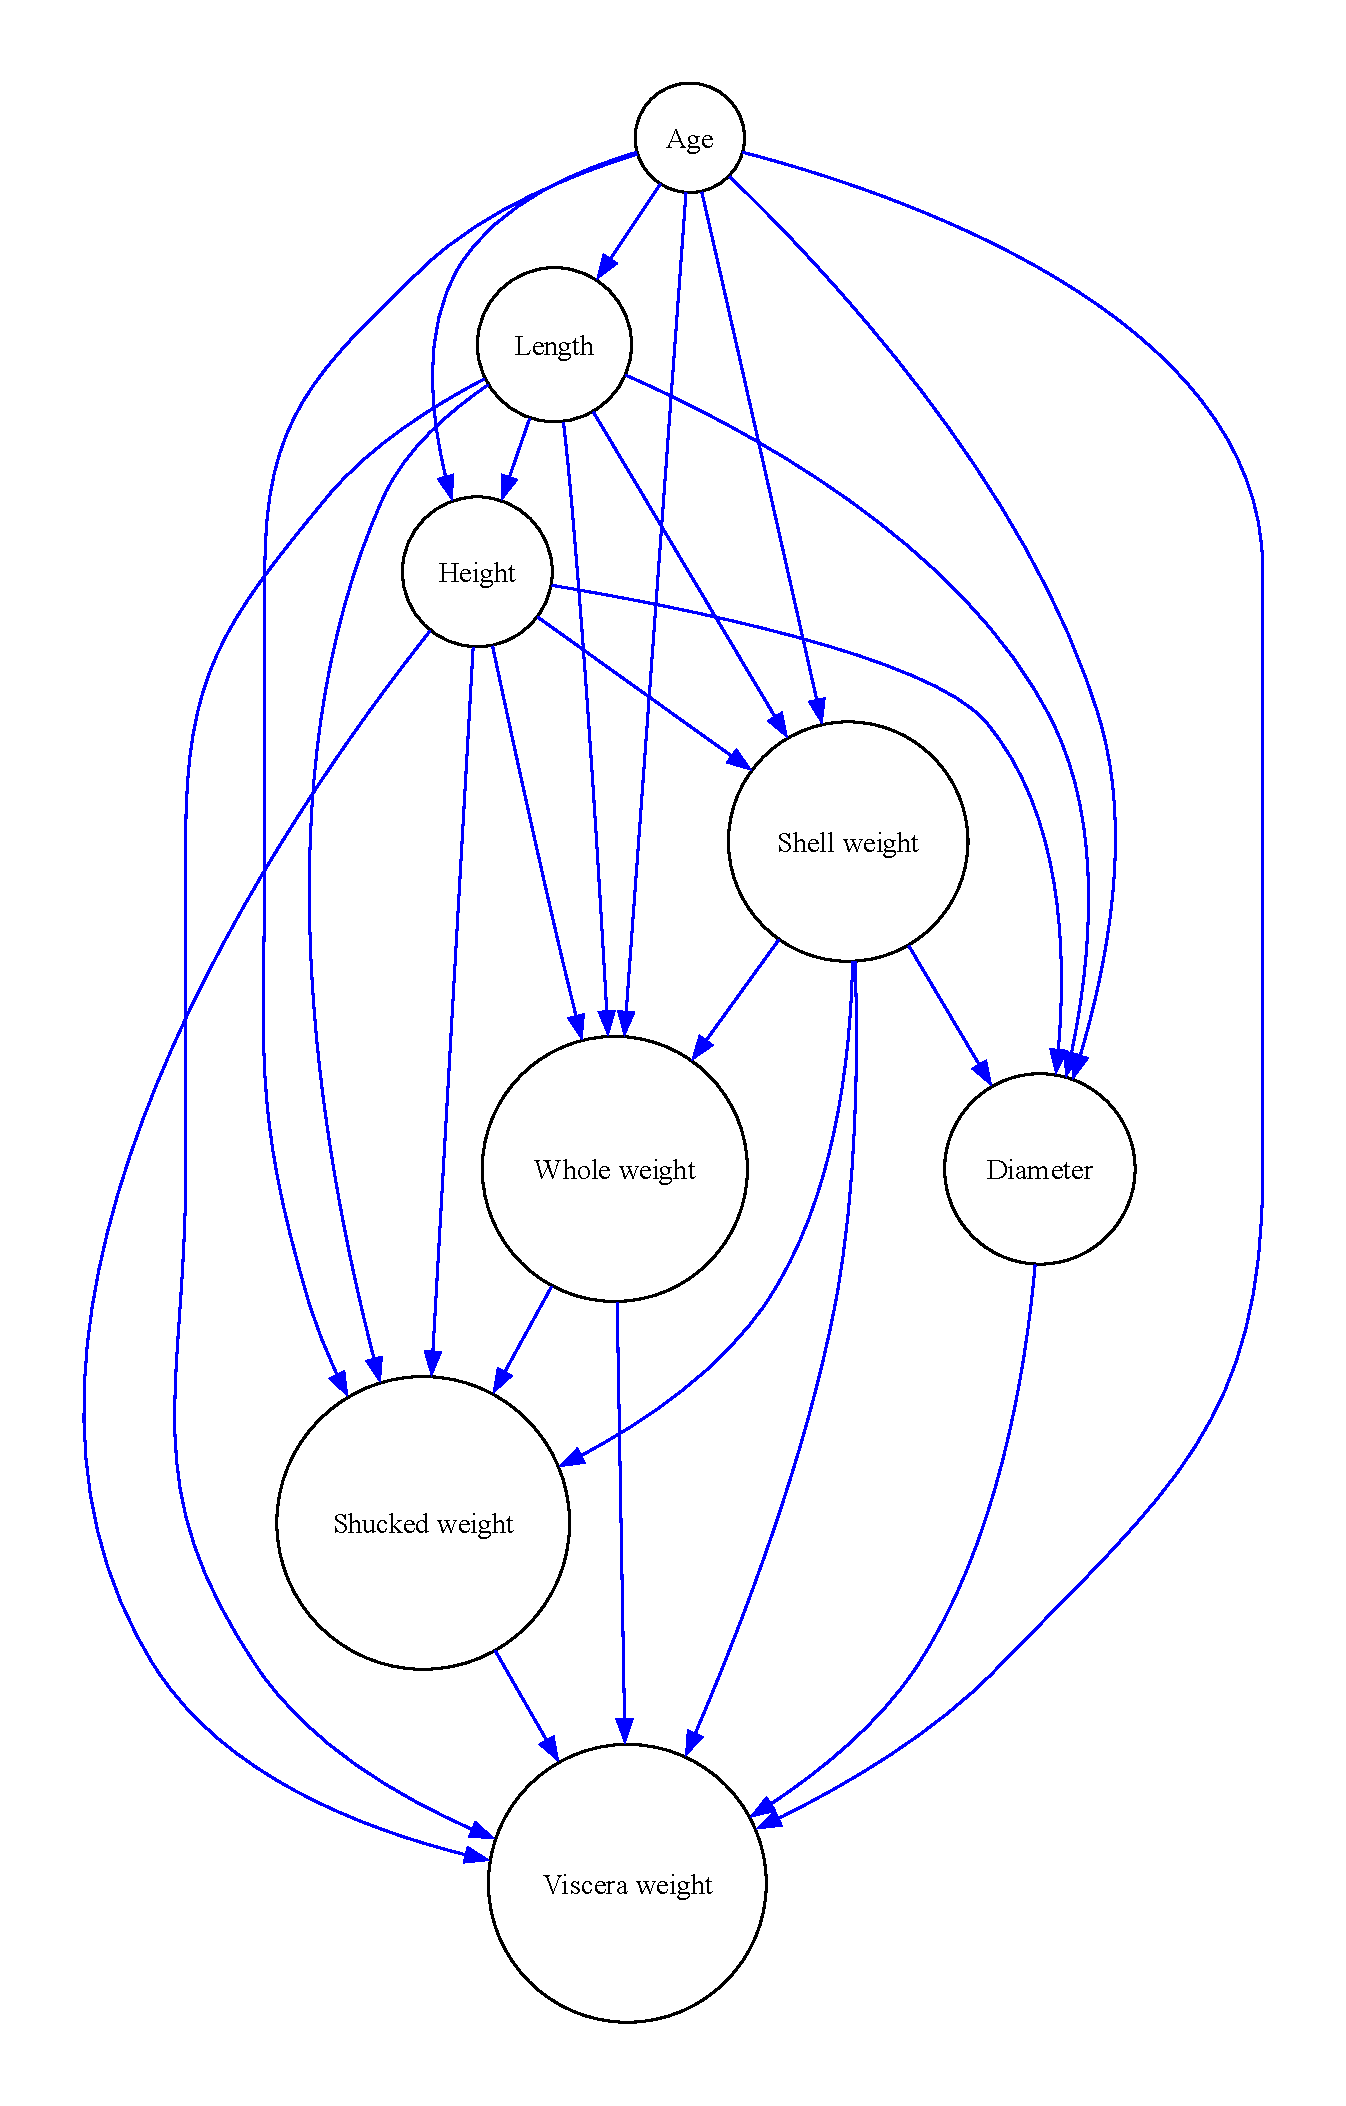
\includegraphics[width=\linewidth]{./demo_data/20241104_132155/Abalone/output_graph/revised_graph.pdf}
        \caption{\label{fig:corr}Revised Graph}
    \end{figure}
\end{minipage}


\subsection{Graph Reliability Analysis}

\begin{figure}[H]
    \centering

\begin{subfigure}{0.32\textwidth}
        \centering
        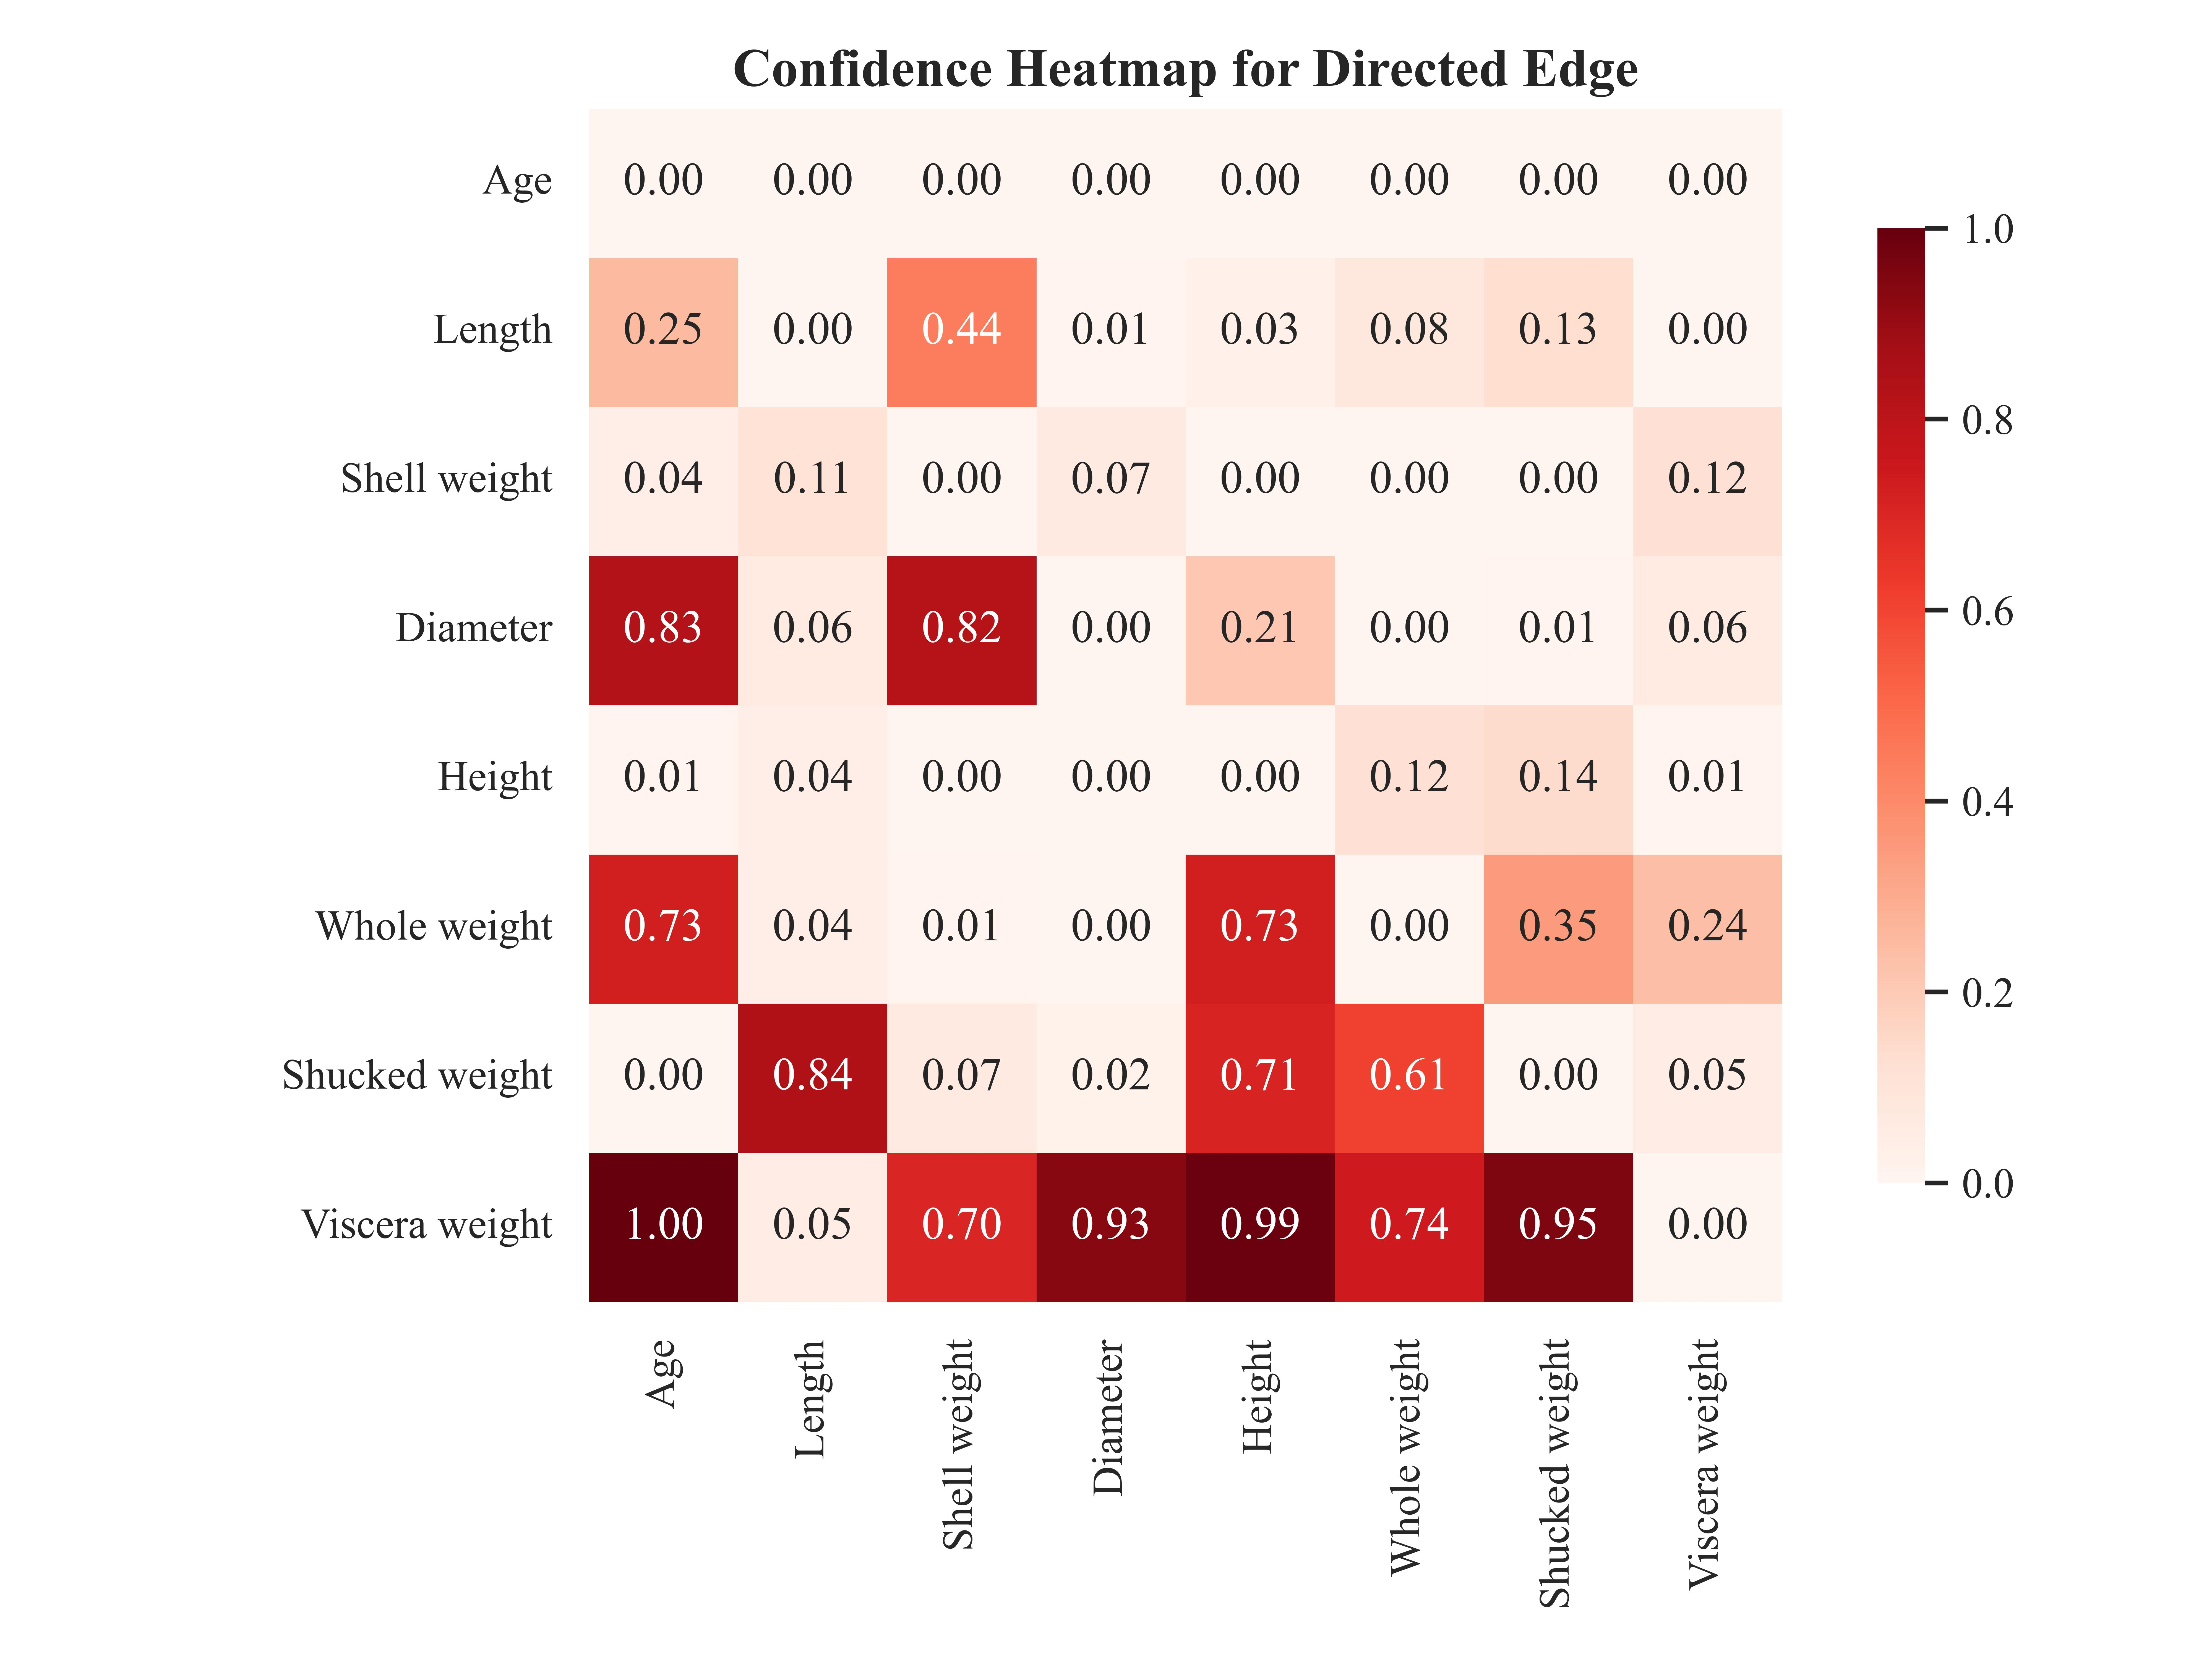
\includegraphics[width=\linewidth]{./demo_data/20241104_132155/Abalone/output_graph/certain_edges_confidence_heatmap.jpg}
        \caption{Directed Edge}
    \end{subfigure}
\begin{subfigure}{0.32\textwidth}
        \centering
        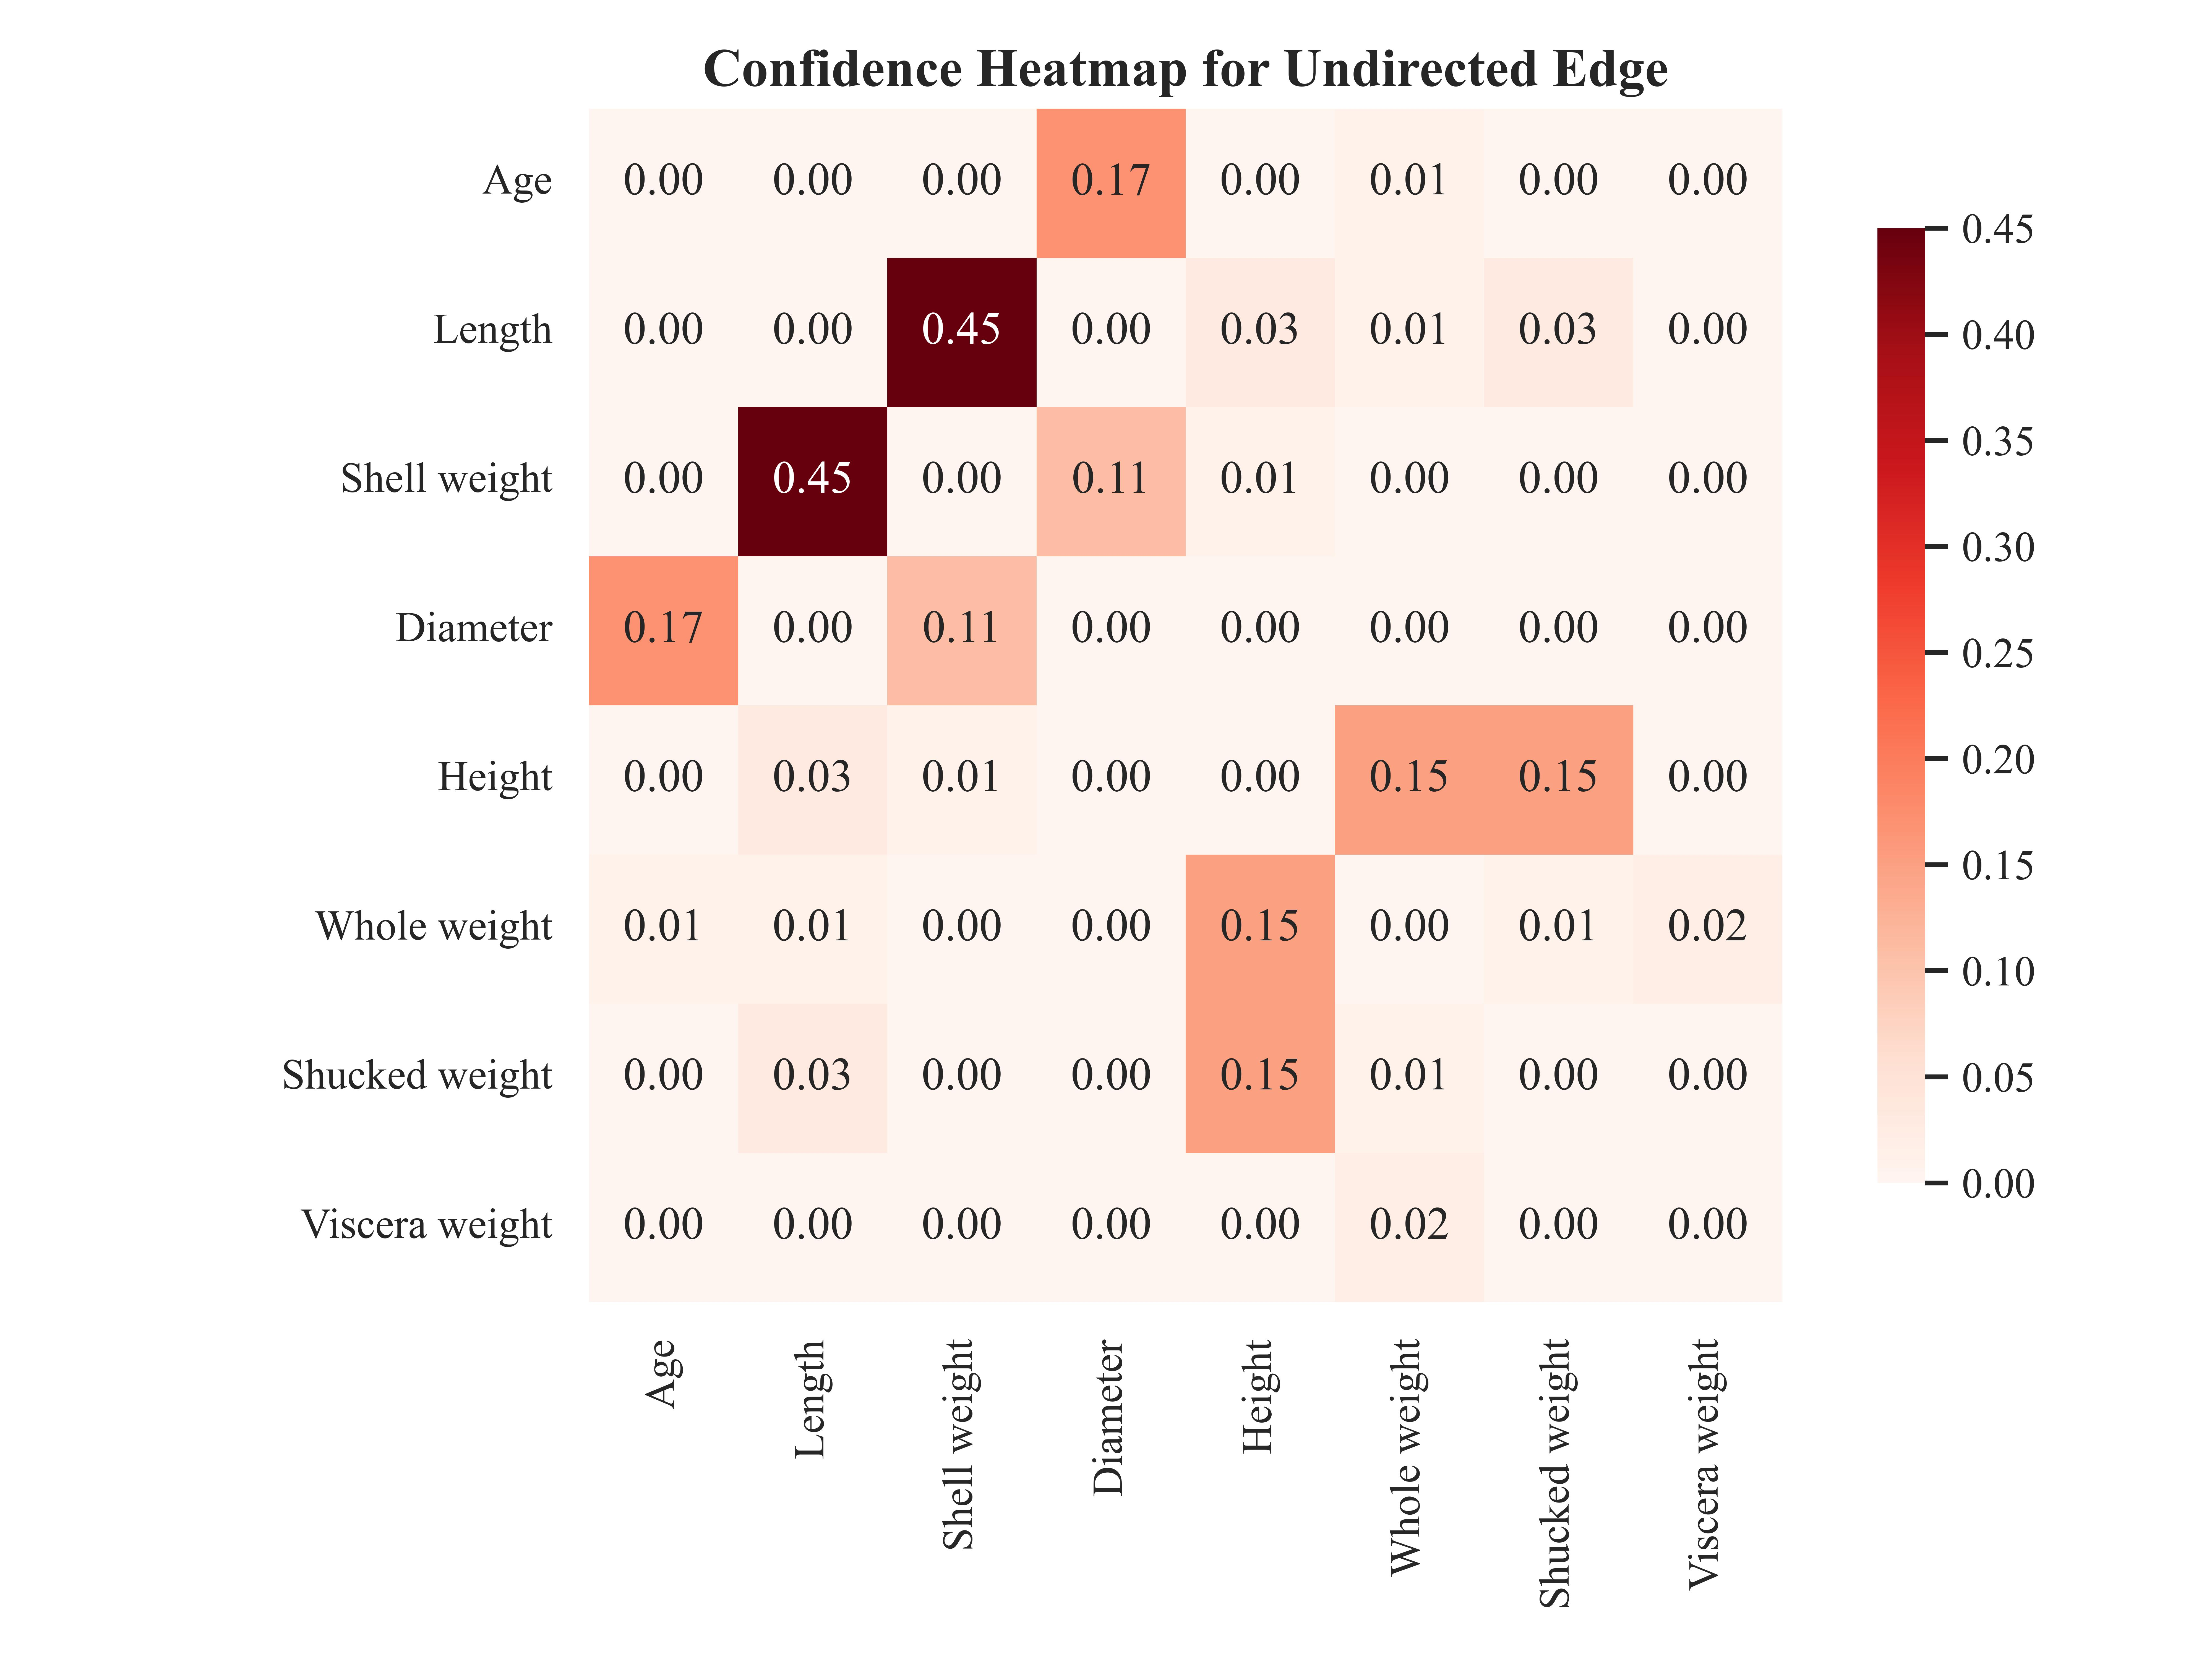
\includegraphics[width=\linewidth]{./demo_data/20241104_132155/Abalone/output_graph/uncertain_edges_confidence_heatmap.jpg}
        \caption{Undirected Edge}
    \end{subfigure}
\begin{subfigure}{0.32\textwidth}
        \centering
        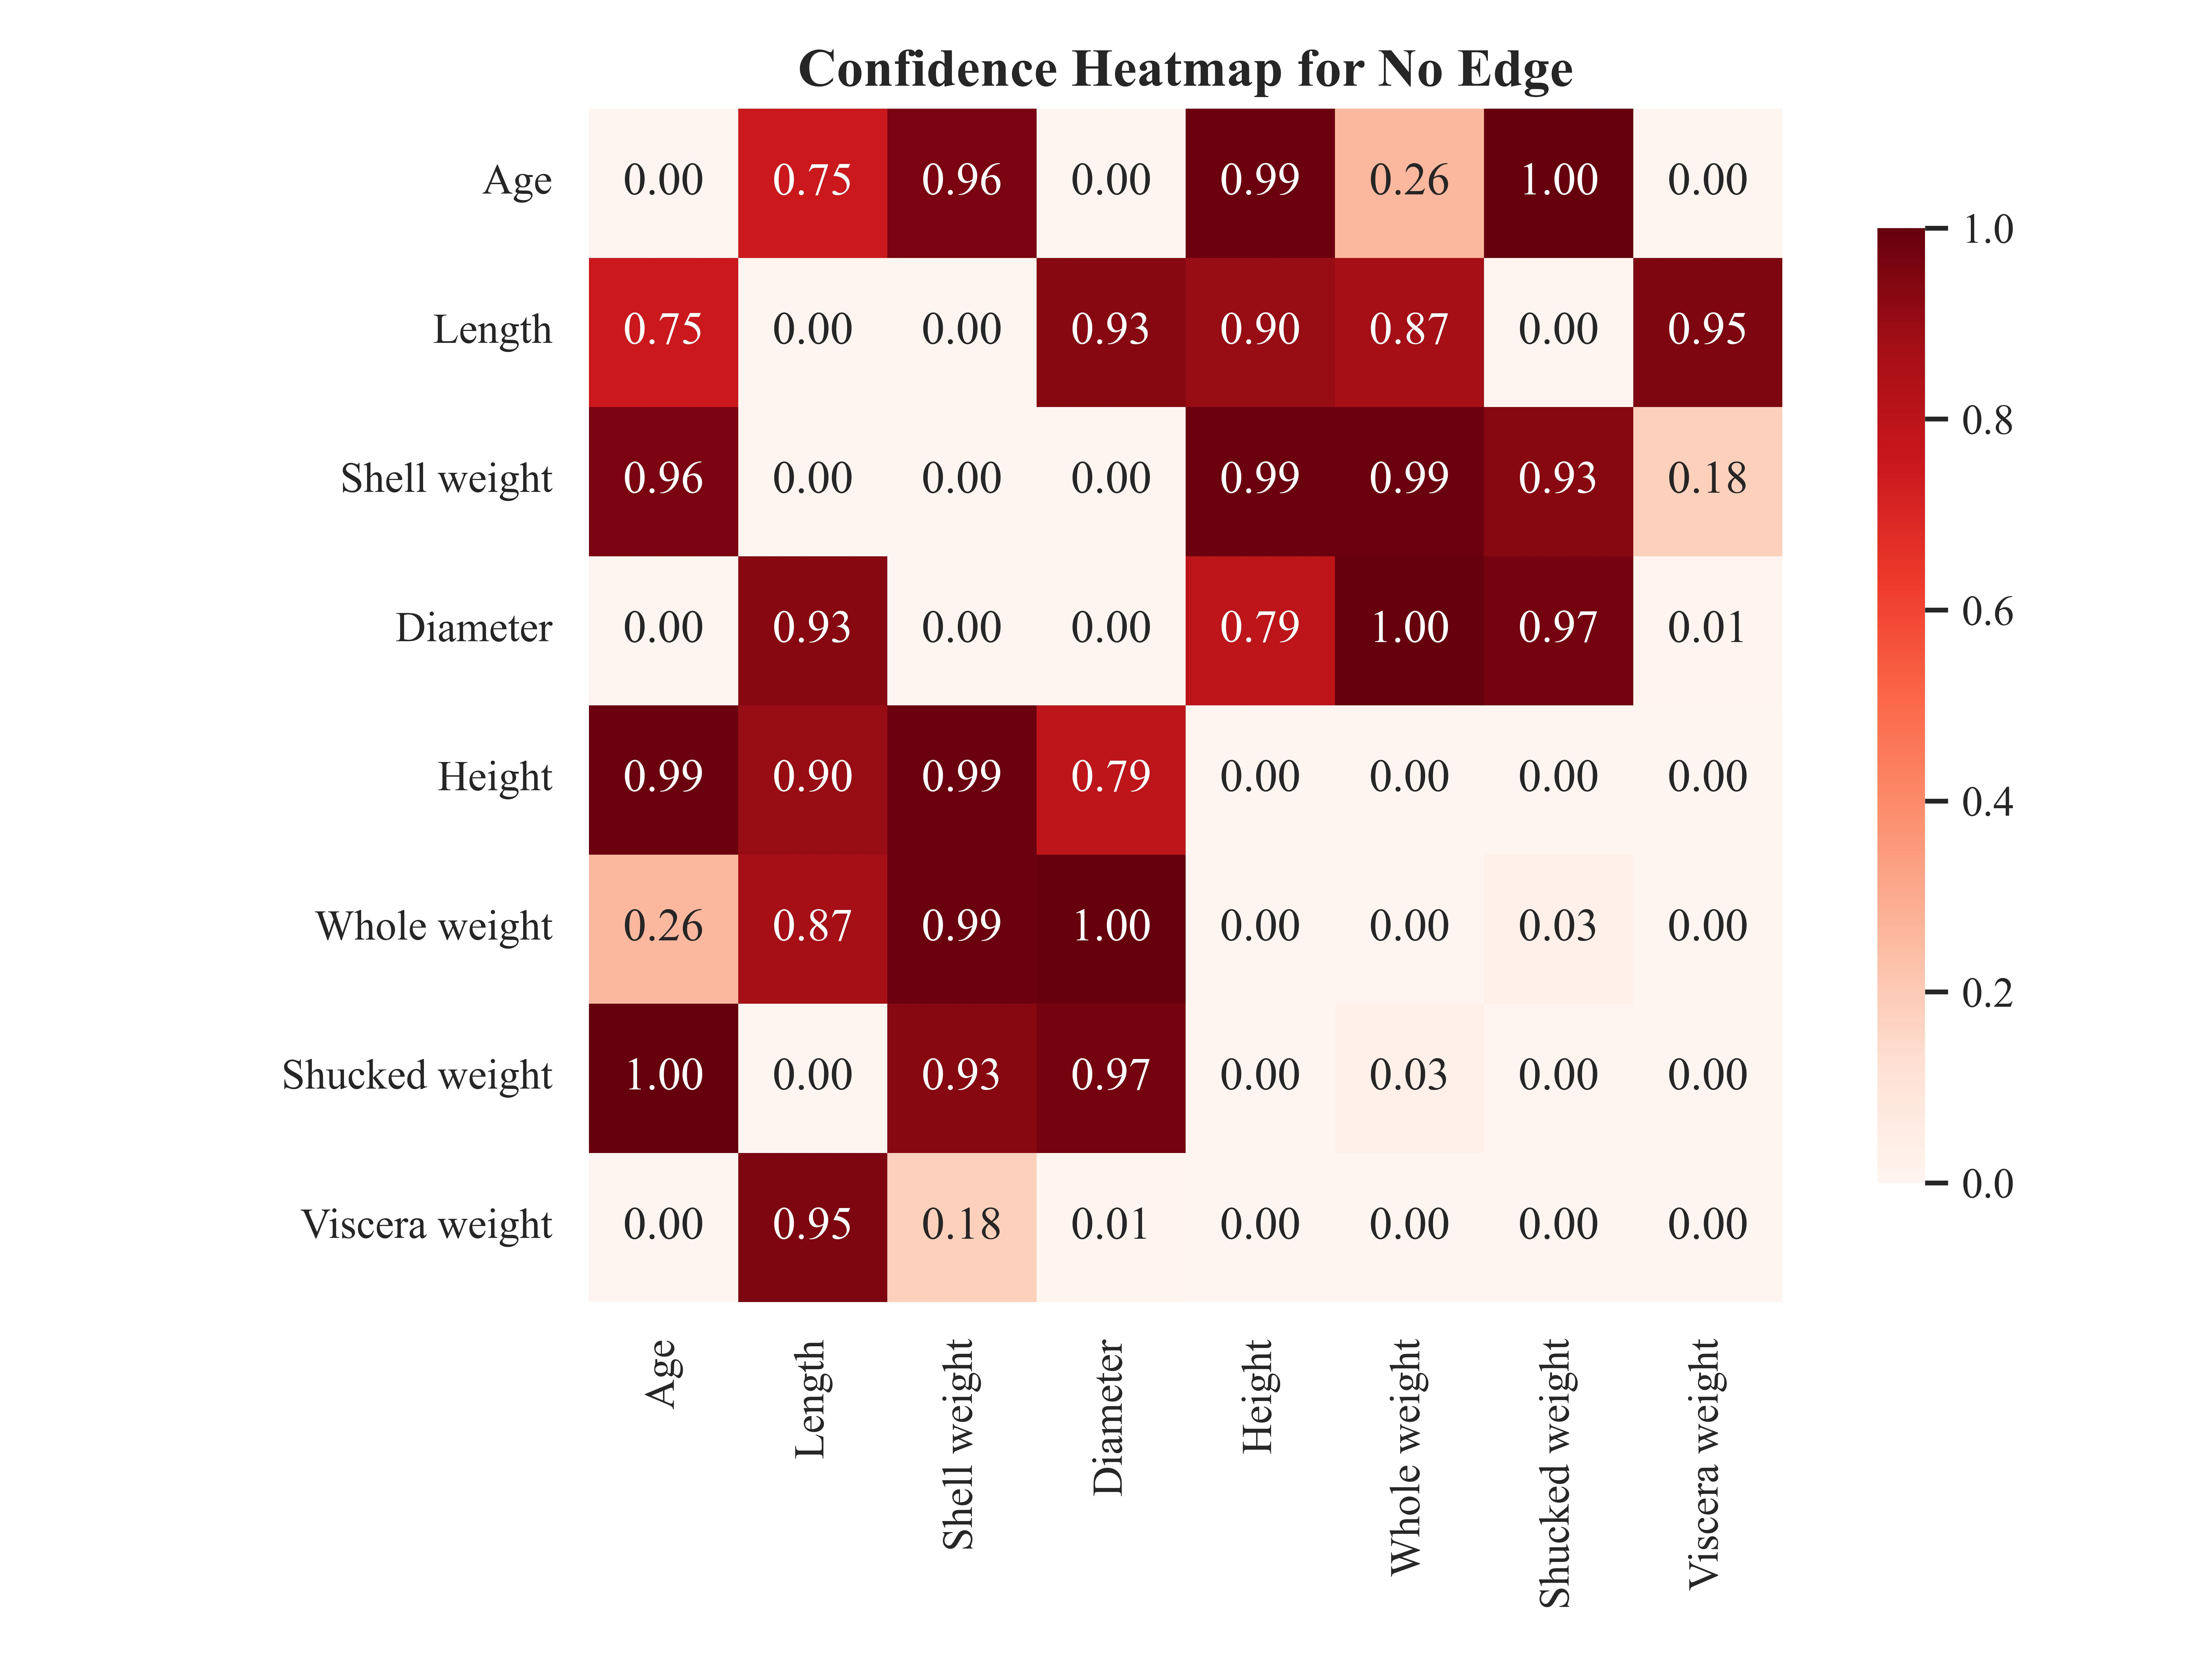
\includegraphics[width=\linewidth]{./demo_data/20241104_132155/Abalone/output_graph/non_existence_confidence_heatmap.jpg}
        \caption{No Edge}
    \end{subfigure}
    \caption{Confidence Heatmap of Different Edges}
\end{figure}        
The above heatmaps show the confidence probability we have on different kinds of edges, including directed edge ($\rightarrow$), undirected edge ($\leftrightarrow$), No Edge, and probability of no edge. The heatmap of bi-edges is not shown because probabilities of all edges are 0. Based on the confidence probability heatmap and background knowledge, we can analyze the reliability of our graph.

From the statistics perspective, we have high confidence to believe that the edges corresponding to the relationships \textbf{Whole weight $\rightarrow$ Height} (bootstrap probability of 0.73) and \textbf{Whole weight $\rightarrow$ Shucked weight} (bootstrap probability of 0.35) exist, as these probabilities indicate considerable confidence in the causal link between these variables. Conversely, we have very low confidence that the edges \textbf{Age $\rightarrow$ Diameter} and \textbf{Age $\rightarrow$ Viscera weight} exist, both having a bootstrap probability of 0.0, which suggests no significant relationship.

However, based on the expert knowledge, we know that the edges \textbf{Age $\rightarrow$ Length, Diameter, Height} and \textbf{Length, Diameter, Height $\rightarrow$ Whole weight, Shell weight} likely exist due to the biological growth patterns of abalones that correspond with aging, thus increasing their size and weight. Conversely, while some edges with low bootstrap probabilities, such as \textbf{Length $\rightarrow$ Shell weight} and \textbf{Shell weight $\rightarrow$ Diameter}, may still represent plausible biological relationships, they lack strong statistical support.

Therefore, the result of this causal graph is partially reliable. While some relationships are supported statistically and align with expert knowledge, the presence of edges with low or no confidence suggests that caution should be taken when inferring causality between those variables. Further investigation and additional data may be needed to enhance the credibility of the proposed causal graph.

\end{document}